\documentclass[xcolor=dvipsnames,hyperref={pdfpagelabels=false}]{beamer}

\usetheme{Boadilla}

\newcommand{\bi}{\begin{itemize}}
\newcommand{\ei}{\end{itemize}}
\newcommand{\be}{\begin{enumerate}}
\newcommand{\ee}{\end{enumerate}}
\newcommand{\bc}{\begin{center}}
\newcommand{\ec}{\end{center}}
\newcommand{\bd}{\begin{description}}
\newcommand{\ed}{\end{description}}
\newcommand{\I}{\item}
\newcommand{\f}{\frame}
\newcommand{\ft}{\frametitle}

\title{Offline Software Overview}
\subtitle{GlueX Collaboration Meeting}
\author[Mark Ito]{Mark M.\ Ito}
\date{October 3, 2014}
\institute[JLab]{Jefferson Lab}

\begin{document}

\f{\titlepage}

\f{\ft{Outline}
\bi
\I Data Challenge
  \bi
  \I goals
  \I conditions
  \I sites
  \I organization
  \I issues
  \I results
  \I outcomes
  \I next
  \ei
\I Other Topics
\I To Do
\ei
}

\f{\ft{Goals}
\bi
\I nominal goal 10 billion events.
\I Pythia/BGGEN events from 7.0GeV to the endpoint.
\I Target distribution to be nominal LH2 as handled by HDGEANT.
\I 1350 A current for magnetic field
\I updated REST format, matching info saved
\I use the CCDB
\I not crash so much
\ei
}
  
\f{\ft{Conditions}
\bi
\I software versions specified
\I background settings \\
\begin{tabular}{|c|c|c|}
\hline
Run & $\gamma$ Rate & fraction \\
\hline
9001 & $1\times 10^7$ & 80\% \\
9002 & $5\times 10^7$ & 5\% \\
9003 & 0 & 15\% \\
\hline
\end{tabular}
\I file number assignments for each site
\I configuration files specified
\I command-lines specified
\ei
}

\f{\ft{Conditions Webpage}
$$
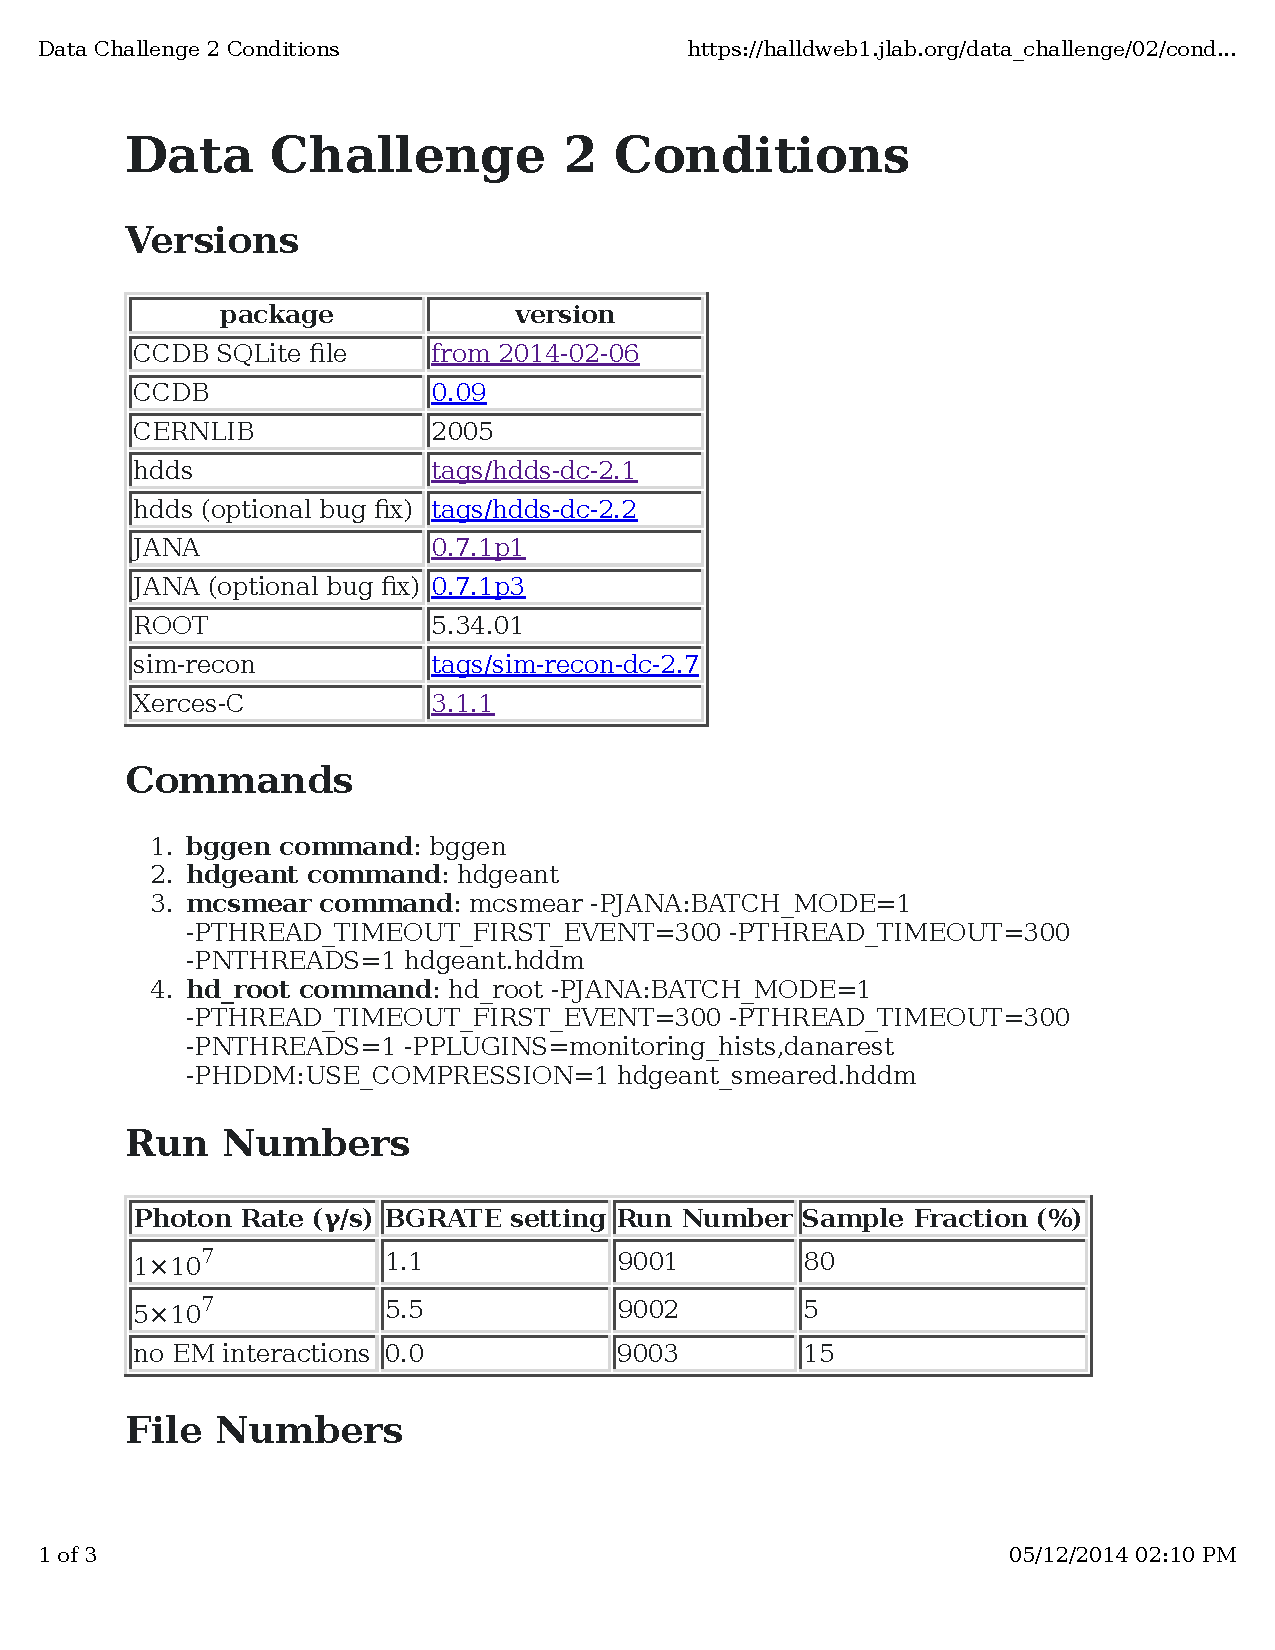
\includegraphics[height=0.9\textheight]{conditions.pdf}
$$
}

\f{\ft{Sites}
\bi
\I Carnegie Mellon
  \bi
  \I 384 cores
  \ei
\I Florida State
  \bi
  \I 144 cores
  \ei
\I JLab
  \bi
  \I 400 to 2400 cores
  \I workflow tools at JLab not ready
  \ei
\I MIT
  \bi
  \I 300+ cores
  \I OpenStack at MIT
    \bi
    \I Virtual Machines instances
    \I MIT Re-Use Cluster
    \I FutureGrid
    \ei
  \ei
\I Open Science Grid (OSG)
  \bi
  \I up to 10,000 cores
  \I nodes contributed from UConn and Northwestern
  \ei
\ei
}

\f{\ft{Organization}
\bi
\I Curtis initiated series of weekly meetings
  \bi
  \I 10 held: January 31 through April 11
  \I in addition to Offline meetings
  \ei
\I conditions webpage
  \bi
  \I Subversion controlled
  \ei
\I Event Tally Board
  \bi
  \I Google Drive spreadsheet
  \ei
\ei
}

\f{\ft{Issues}
\bi
\I reversed magnetic field fixes from Simon
\I Kei studied effect of EM background on file size, and execution time, varying beam rate and gate length
\I phi = 0 problem in CDC solved, Richard, Simon
\I event geneology checked by Kei
\I fix from Simon for single-ended TOF counters
\I improvements from Paul for cutting off processing for multi-lap curling tracks, big memory footprint effect
\I ZFATAL fix from richard, showers from EM background, squelched
\I short REST file fix from richard: bug in xstream library with compression enabled
\I non-reproducibility fixed: sort needed on associated objects in STL map
\ei
}

\f{\ft{Issues (continued)}
\bi
\I random number seeds
  \bi
  \I looked at scheme where every event stores its seed at each stage
  \I settled on bggen seed; concession to GEANT random number generator
  \ei
\I Kei studied EM background effect for $p\pi^+\pi^-$, $p\pi^+\pi^-\pi^0$
\I enhanced job tracking info at JLab added, MMI
\I Python script to scan monitoring histograms from Sean
\ei
}

\f{\ft{Results}
\bi
\I code frozen on March 20
\I events produced: more than 8 billion
\I execution time \\
\begin{tabular}{|c|c|c|}
\hline
Run & $\gamma$ Rate & sec/event \\
\hline
9001 & $1\times 10^7$ & 2.4 \\
9002 & $5\times 10^7$ & 9.0 \\
9003 & 0 & 0.75 \\
\hline
\end{tabular}
\I memory usage: about 1 GB peak virtual memory
\I reliability:
  \bi
  \I CMU: 7000 jobs, 3 failures
  \I JLab: 69,000 jobs, about 50 failures
  \ei
\I JLab node history:
  \bi
  \I Hall D share from 360 to 440 to 1440 to 2440
  \I Million core hours owed to us, cores lent to lattice QCD cluster
  \ei
\I non-OSG sites ramped down April 11 plus or minus a few days (last data challenge meeting)
\ei
}

\f{\ft{Event Tally Board}
$$
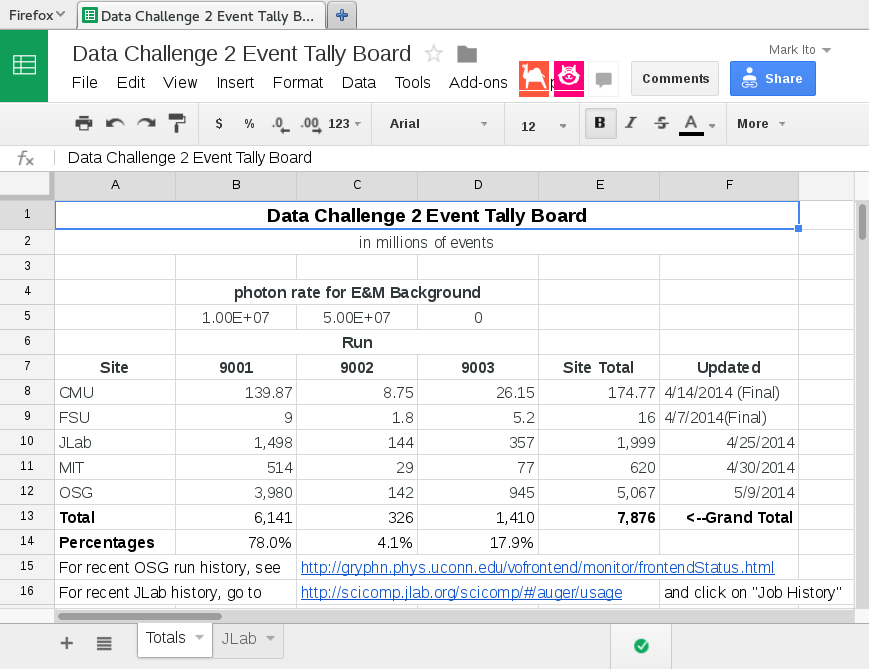
\includegraphics[width=0.9\textwidth]{event_tally_board.png}
$$
}

\f{\ft{JLab Farm Usage}
$$
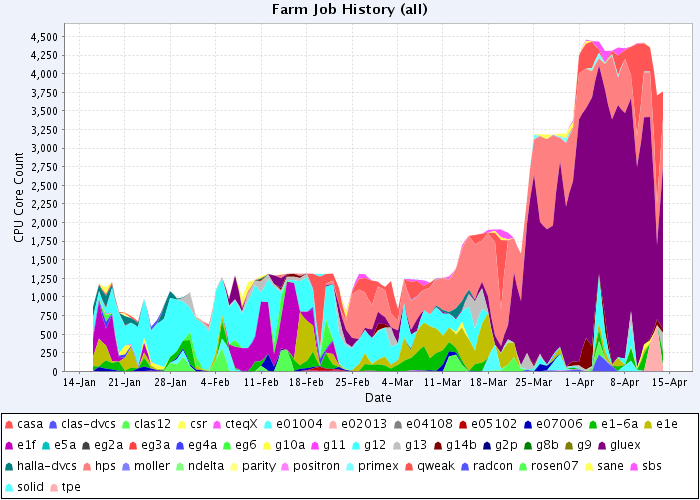
\includegraphics[width=0.9\textwidth]{Farm_2014.png}
$$
}

\f{\ft{MIT OpenStack Jobs}
$$
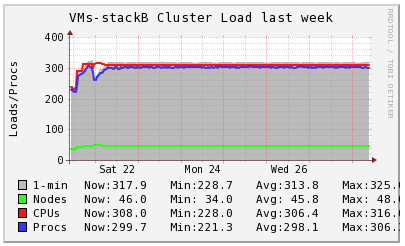
\includegraphics[width=0.9\textwidth]{MIT_DC2_3-28-14.png}
$$
}

\f{\ft{CPU Time Usage (Jlab)}
$$
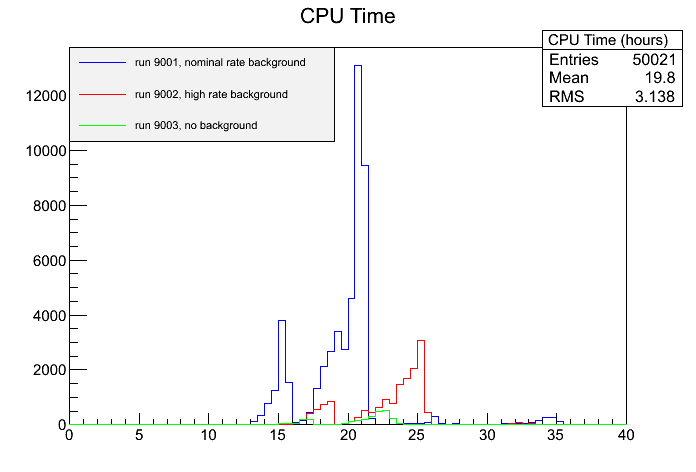
\includegraphics[width=0.9\textwidth]{cput.png}
$$
}

\f{\ft{Virtual Memory Peak (JLab)}
$$
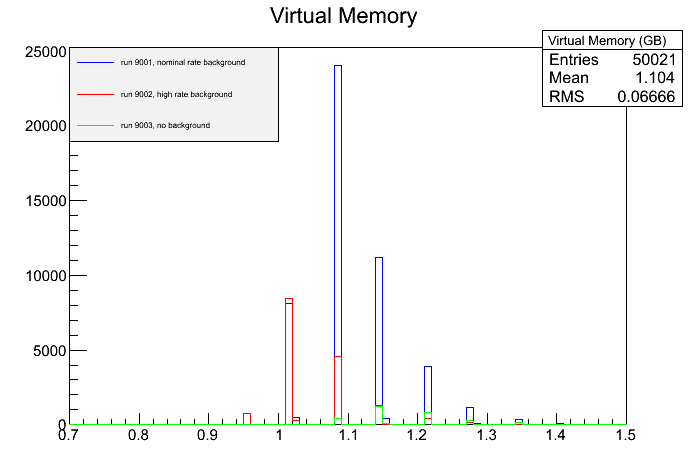
\includegraphics[width=0.9\textwidth]{vmem.png}
$$
}

\f{\ft{Data Distribution}
\bi
\I Storage Resource Manager (SRM)
  \bi
  \I go-to method for shipping data between sites
  \I archiving all data to tape library at JLab now
  \ei
\I EventStore
  \bi
  \I Sean developing this
  \I Multiple skim available from single data file (REST)
  \I Managing event lists
  \ei
\I Paul developed menu of skims we might do
\ei
}

\f{\ft{What Came Out}
\bi
\I need more efficient EM background generation scheme
\I large usable data set (hopefully)
\I improvements of techniques at various sites
\I need a monitoring system for production (ROOTSpy?)
\I need for Geant4
\ei
}

\f{\ft{Next Data Challenge}
\bi
\I stage ``raw data'' on tape library
\I ``production''
\I tape overhead
\I test multi-threading
\I needed: raw data, ability to analyze it
\I summer?
\ei
}

\f{\ft{Other Topics}
\bi
\I CCDB 1.00 released
\I kinematic fitter update
\I nightly build using scons
\I BlueJeans deployed
\I splitting up offline packages
\I re-org of offline wiki pages
\ei
}

\f{\ft{Conclusions}
\bi
\I much more robust software suite coming out of data challenge
\I high level of cooperation and coordination demonstrated
\I lots to do
\I next frontier: reconstruction quality
\ei
}

\end{document}

May 28
* NU files not copied yet
* David produced new field maps
* Sean has the backend database code for EventStore all done
* David told us about a change he made to CCDB so that one-dimensional arrays treated the same whether they are one-row-by-many-columns or many-columns-by-one-row
June 11
* Zisis commented on the state of the software getting-started documentation on the wiki
* Simon has changed the code to get the parameter for the minimum number of hits on a track candidate from a JANA configuration parameter. Formerly it was hard-wired at 6. 
* David brought us up-to-date on the status of doing reconstruction with EVIO data derived from simulation output.
* Will explained in more detail the mystery he sees in the simulation output (scroll down to the attachment) that is likely responsible for a late tail in the BCAL time distributions for pions
June 25
* Data Challenge 3
** process fake raw data resident in the tape library
** render the data in EVIO format
** perform more efficient generation of the electromagnetic background
** use the Geant4 version of HDGeant
** incorporate new code for obtaining constants from the CCDB
July 9
* Tagger Reconstruction: Richard led us through his proposal for introducing a random global time offset to all events, consistent with the 500 MHz RF time structure. This would simulate the real-life uncertainty due to event-to-event trigger latency variations and the intrinsic jitter due having a fully pipelined data acquisition system driven on a 250 MHz clock. At present, all events are analyzed as if the true RF bucket is known, a priori. Also the true beam photon energy is also assumed in the analysis. 
* Reinstating the Separation between Truth and Hit Information in HDDM
** Richard described the structure in HDDM that we have now where Monte Carlo truth information is recorded in parallel with "hit" or "detected" information in HDDM in mcsmear. He is implementing these schemes for some additional detectors, including the start counter and the tagger.
** In the process, he is modernizing the HDDM parsing code to use the C++ API rather than the original C routines. This gives a major reduction in lines of code. Also compression will be done on the HDDM output. 
July 23
* The solution is to use the MD5 check-sum that is generated and downloaded along with each resource file to check file integrity each time the file is read. David is working on implementation for the next version of JANA. 
* Haswell CPU Testing: David reported on tests he has done bench-marking a demo machine that SciComp had on loan for this purpose. He compared the demo Haswell machine with an Ivy Bridge gluon machine in the Counting House. 
* Paul has prompted Mark to take up work again on a global build system for GlueX. Paul would like to see multiple versions of each package co-exist in the tree with dependencies among them taken care of. 
* Richard requested that someone convert the build of hdds from GNUMake to scons. David agreed to look into what is involved. 
August 6
* Paul has made the changes to the analysis library to work with the new smeared tagger time, although for now he is cheating by taking the true tagger hit. This is useful for now to establish that the branch will work as before, when indeed this exact cheat was in, once the branch changes are put on the trunk. 
Offline Commissioning
* Sean called our attention to the tasks outlined for the offline in the commissioning plan. We need to add content to this page. We discussed the issue of overlap of this task list with the efforts of the individual detector groups during commissioning, but for the mid-level and high-level tasks the offline has clear responsibility. 
August 20
* Tagger Simulation Update
** HDDM Calls: Conversion to C++ API: All invocations of the HDDM API have been upgraded to use the C++ version rather than the old C version. This change comes in many places in the sim-recon tree. The exception is the GEANT-3-based code, in particular the current HDGeant; that conversion will come with the conversion to Geant4.
** HDDM Integrity Checks: The HDDM library now supports "integrity checks" where a cyclic redundancy check (CRC) code is computed event-by-event and can be written with the event. Downstream programs can check that incoming data has not been corrupted.
** HDDM_s Changes: The template for simulation output has been changed to rationalize the arrangement of data in two areas: (1) the mix of truth and hit information and (2) the detector component hierarchy. A generic example of the latter is using enclosing elements to indicate "layer" rather than encoding "layer" as an attribute of each hit. Note that changes of this nature are indicated in the HDDM_s version in the template contained in every data file.
** Merging Strategy: As he has been making these changes, Richard has been periodically merging changes made to the trunk onto his branch. In this way integration testing can proceed on the branch before merge of the branch back onto the trunk.
** Tagger Analysis: CCDB tagger tables have been rationalized and new C++ classes introduced in sim-recon to accommodate the new scheme. The start counter was used as a model for the low-level hit classes in the DAQ plug-in. There were some modifications needed to HDGeant (GEANT3) code to write the new classes.
** Analysis Library Changes: Paul will need to change the analysis library to deal with the ambiguity of the "correct" tagger hit. For now he will use the factory tag for the tagger to get the true tagger hit. That makes things more or less as things were before. Once the merge onto the trunk is done, he will implement the necessary changes.
gxtwist: Gxtwist is a stand-alone simulation of the tagger hall. Richard has updated the geometry based on the latest drawings. This has been checked in on the trunk. He has also added reality to the radiator with separate positions for the diamond and the amorphous radiators. 
* Re-Creating Tracks: There was a discussion on the email list about re-creating tracks with mass hypotheses that are not present in the set coming from track reconstruction. This can be very time-consuming. In these cases usually the fit failed when using the mass assumption in question. Simon is working on solving this problem in tracking so a full set of mass hypotheses are available in the REST file. See the email discussion for details. 
* Commissioning Geometry Simulation: An effort has started by Sean and Simon to simulate the detector with the commissioning geometry. A branch of HDDS has been made for this work and Simon has started putting in the commissioning target. 
* Analysis of Six Final States Using Data Challenge 2 MC: Ryan has looked at the following reactions generated in Data Challenge 2:

    \gamma p \rightarrow \pi^+\pi^- p
    \gamma p \rightarrow \pi^+\pi^-\pi^0 p
    \gamma p \rightarrow K^+K^- p
    \gamma p \rightarrow \pi^+\pi^-\pi^+\pi^- p
    \gamma p \rightarrow \pi^+\pi^-\pi^+\pi^-\pi^0 p
    \gamma p \rightarrow \pi^+\pi^-\pi^+\pi^-\pi^+\pi^- p 

September 3
* In the context of Ryan's presentation on multi-pion final states, Matt commented that he, Ryan, and Paul did a detailed comparison of Ryan's software and Paul's analysis library, down to comparing single events. With a lot of back and forth to clarify/resolve differences the agreement between the two is "perfect in some very difficult to reproduce, slightly obscure way".
* Simulating the Commissioning Geometry
** Simon is done with putting in the geometry changes associated with the commissioning configuration. He as not done a check for overlaps yet.
** Sean is putting together a set of configuration files do drive large-scale simulation using this geometry. Simon has done some tests as well. 
* Comparing Simulated HDDM and EVIO Files: Sean has done comparisons between hit information between simulation native output (HDDM format) and EVIO data derived from same using the new trunk from Richard (see above).
September 17
* DC3: With all of the activity centered around the commissioning run, Mark was skeptical if he and others have the time to fully launch Data Challenge 3 at this time. Its start will likely be delayed a month or so. 
* Offline Analysis of Online Data and Coordination Thereof: Paul has volunteered to organize this effort. 
* Monitoring Histograms: David and Sean will work on documenting the process for implementing online monitoring histograms. These are done with plugins and use ROOTSpy to collect statistics from multiple nodes. Elliott Wolin started this effort, but it there have been changes in recent weeks. Sean also has done some development on the ROOTSpy package, as has David. 
